\paragraph{Protocol.} The configuration (two bands, discrepancy $\kappa=0.5$, GP length scale 5\,d) was chosen on the validation split by a preregistered rule, and five hypotheses were fixed: P is less often confidently wrong than B3 on unmodeled events (H1); $P(h_0)$ ranks unmodeled above modeled events (H2, AUROC $>0.5$); P is not more than 5 points more often confidently wrong than B3 on supernovae (H3) and not more than 5 points less accurate (H5); and colour raises the AUROC over a single-band arm on the same events (H4). Each must pass on all three noise seeds (stratified paired bootstrap, $10^4$ resamples). The test events (\RealNEvents: \RealNModeled\ supernovae, \RealNWithheld\ unmodeled) had been used twice before, in the retrospective analyses; this causal run is a declared third look.

\paragraph{Results.} Table~\ref{tab:real} gives both versions side by side. With causal measurements, H1--H4 pass and H5 fails. Closed-world EIG was confidently wrong on \RealCCwWhBthree\ of real unmodeled transients (retrospectively \RealRCwWhBthree), the auction baseline B1 on \RealCCwWhBone, and P on \RealCCwWhP. P labelled \RealCFlagP\ of unmodeled events as unknown, and its AUROC was \RealCAuc\ (Fig.~\ref{fig:rocreal}).

\begin{table*}[t]
\centering\scriptsize
\caption{Real ZTF replay, preregistered test results per noise seed: estimate [95\% CI]; $^\times$ = criterion not met on that seed. CW: confident-wrong rate; $\Delta$ = P minus B3, or colour minus single-band arm for H4. Causal (v3) is this paper's result; retrospective (v2) let planners measure earlier epochs after later ones and is shown for comparison only.}
\label{tab:real}
\begin{tabular}{lll@{\hspace{4pt}}l}
\toprule
& Seed & Causal (v3) & Retrospective (v2) \\
\midrule
H1 $\Delta$CW unmod. & 1 & -0.49 [-0.60, -0.36] & -0.60 [-0.72, -0.49] \\
 & 2 & -0.42 [-0.55, -0.30] & -0.67 [-0.77, -0.56] \\
 & 3 & -0.36 [-0.48, -0.25] & -0.60 [-0.73, -0.48] \\
\addlinespace
H2 AUROC $P(h_0)$ & 1 & +0.81 [+0.76, +0.86] & +0.80 [+0.75, +0.85] \\
 & 2 & +0.81 [+0.76, +0.86] & +0.80 [+0.75, +0.85] \\
 & 3 & +0.79 [+0.73, +0.84] & +0.77 [+0.71, +0.82] \\
\addlinespace
H3 $\Delta$CW mod. & 1 & -0.05 [-0.09, -0.01] & +0.00 [-0.06, +0.07]$^\times$ \\
 & 2 & -0.04 [-0.08, +0.00] & +0.04 [-0.03, +0.10]$^\times$ \\
 & 3 & -0.03 [-0.07, +0.01] & +0.06 [-0.01, +0.12]$^\times$ \\
\addlinespace
H4 $\Delta$AUROC colour & 1 & +0.19 [+0.13, +0.24] & +0.19 [+0.14, +0.24] \\
 & 2 & +0.18 [+0.12, +0.23] & +0.21 [+0.16, +0.27] \\
 & 3 & +0.24 [+0.18, +0.30] & +0.15 [+0.10, +0.20] \\
\addlinespace
H5 $\Delta$acc.\ mod. & 1 & +0.01 [-0.05, +0.07]$^\times$ & -0.08 [-0.14, -0.02]$^\times$ \\
 & 2 & +0.03 [-0.04, +0.09] & -0.06 [-0.13, +0.00]$^\times$ \\
 & 3 & -0.01 [-0.08, +0.05]$^\times$ & -0.08 [-0.14, -0.01]$^\times$ \\
\addlinespace
\bottomrule
\end{tabular}

\end{table*}

\begin{figure}[t]
\centering
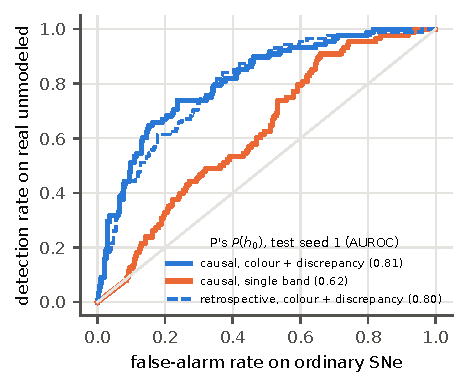
\includegraphics[width=\columnwidth]{generated/figures/fig4_roc_real.pdf}
\caption{Real data: ROC of the open-world planner's $P(h_0)$ separating real unmodeled transients (TDE, SLSN, SN~Ibn) from ordinary supernovae, test seed 1. Colour plus model discrepancy is what makes $h_0$ usable; enforcing causality leaves the curve almost unchanged.}
\label{fig:rocreal}
\end{figure}

\paragraph{What causality changed.} The retrospective runs failed H3 and H5: P paid for its safety on unknowns with more confident errors and lower accuracy on ordinary supernovae. Causally, H3 passes, the false-``unknown'' rate on supernovae falls from \RealRFaP\ to \RealCFaP, and P's supernova accuracy (\RealCAccModP) matches B3's (\RealCAccModBthree). H5 still fails, narrowly: on two seeds the lower confidence bound falls just below $-5$ points, so we cannot rule out a small loss. The cost moved to the unknowns: P flags \RealCFlagP\ of them, against \RealRFlagP\ retrospectively. The mechanism is the measurement budget. With a time arrow, one-step utilities jump to a late, informative epoch and forfeit the earlier ones: P used \RealCObsP\ of its 5 measurements on average (B3 \RealCObsBthree, the fixed-cadence B0 \RealCObsBzero), against \RealRObsP\ when it could go back in time. Fewer measurements make every posterior less confident, which removes confident errors on both populations, and with them some of P's detections.
